%\documentstyle{llncs}
%\documentclass[12pt,fullpage]{llncs}
\documentclass[12pt]{article}
%\usepackage[left=3cm,top=1.2cm,right=3cm,nohead,nofoot]{geometry}
%\usepackage[letter,left=.25in,right=.25in,top=.17in,textwidth=7.5in,textheight=9in]{geometry}
%\usepackage[left=0cm]{geometry}

%\documentclass[12pt]{report}
%\usepackage {utthesis2}              %% Preamble.

%\usepackage{amsmath}
%\usepackage{amssymb}
\usepackage{arabtex}
\usepackage{amsmath}
\usepackage{amssymb}
\usepackage{times}
\usepackage{caption}
\usepackage{epsfig}
\usepackage{subfigure}
\usepackage{color}
\usepackage{rotate}
\usepackage{rotating}
\usepackage{multirow}
%\usepackage[colorlinks=false]{color,hyperref}
\usepackage{color,hyperref}
%\usepackage{amsthm}
\usepackage{booktabs}
\usepackage{multirow}
\usepackage{natbib}
\bibpunct{[}{]}{,}{n}{}{;}

\usepackage{url}

\usepackage{relsize}
\usepackage{fancyvrb}
\usepackage{fancyhdr,lastpage}

\usepackage{utf8}
\setarab
\fullvocalize
\transtrue
\arabtrue

\newcommand{\CharCodeIn}[1]{`\CodeIn{#1}'}
\newcommand{\CodeIn}[1]{{\small\texttt{#1}}}
\newcommand{\frl}[1]{\fbox{\RL{#1}}} 
\newcommand{\noArRL}[1]{\arabfalse\RL{#1}\arabtrue} 
\newcommand{\noTrRL}[1]{\transfalse\RL{#1}\transtrue} 
\newcommand{\noTrNoVocRL}[1]{\novocalize\transfalse\RL{#1}\transtrue\vocalize} 
%\newcommand{\drawline}{\begin{picture}(6,.1) \put(0,0) {\line(1,0){6.25}}\end{picture}}

\usepackage{setspace}
%\doublespacing
\renewcommand{\baselinestretch}{1.15}
\setlength{\parindent}{0in}
%\parskip 6pt
%\parindent 0pt
%\setlength{\parskip}{.05in}
%\oddsidemargin 0in
%\evensidemargin 0in
\oddsidemargin .0in
\evensidemargin .0in
\hoffset -.75in
\voffset -.83in
\textwidth 7.5in
\textheight 9.5in

\topsep 0in
\topmargin 0.17in

%\usepackage{arabtex}
%\usepackage{utf8}

\begin{document}


\pagestyle{fancy}
%\lhead{}
\chead{}
\rhead{}

\lfoot{LNCSR Progress Report}
\cfoot{}
\rfoot{Page \thepage~of~\pageref{LastPage} }
\renewcommand{\footrulewidth}{0.2pt}
\renewcommand{\headrulewidth}{0.2pt}

%\begin{titlepage}

\begin{center}
{\Large \bf Relational Queries \\
for Arabic Text Mining }

%\setlength{\unitlength}{1in}
%\setlength{\unitlength}{1in}
\vspace{1.5in}

\renewcommand{\arraystretch}{.6}
\begin{tabular}{cc}
Fadi Zaraket \\
Electrical and Computer Engineering  \\
American University of Beirut \\
{\tt fadi.zaraket@aub.edu.lb} 
\end{tabular}

\vspace{1.5in}

\renewcommand{\arraystretch}{.6}
\begin{tabular}{c}
{\small Research Progress Report } \\
{\small Submitted to }\\
\\
    Lebanese National Council for Scientific Research \\
    (LNCSR)
\end{tabular}
\vspace{.5in}

\date{\today}
\pagebreak

\end{center}


In this report we discuss our progress and work on the 
{\bf Relational Queries for Arabic Text Mining} project 
funded by LNCSR.
\\

This document is organized as follows:
\begin{enumerate}
\item Summary of work conducted during the first year of the project
\item Goals for next year
\item Budget for year 2011
\item Attached submission to ``ACL/HTL 2011"
\end{enumerate}
\pagebreak

\section{Summary of work conducted during the first year of the project}
\label{s:prelim}

At the American University of Beirut (AUB), we
started work on an Arabic text mining framework~\cite{ATMine09}
that is available now online. 
ATMine is around 20K lines of C++, perl, and sql code and uses 
middleware from the open source community such as MySQL, Qt, and 
double array trie.


Arabic morphological analyzers~\cite{Sughaiyer:04}
consider an Arabic word and its internal structure composed of 
several {\em morphemes}. 
A morpheme is a {\em stem} or an {\em affix}.
An affix is a {\em prefix, suffix,} or an {\em infix}.
The analysis of one word may lead to several possible
solutions.
\vocalize
For instance, the word 
\RL{'a.hmadH}~\footnote{In this document, we use the default 
ArabTeX transliteration style ZDMG.}
may have two valid morphological analyses. 
The word means ``I praise him'' when
the letter \RL{'a} is a prefix and  it means
``his Ahmad'' when 
the letter \RL{'a} is part of the proper noun stem 
\RL{'a.hmad}.

Current morphological analyzers such as 
Buckwalter~\cite{Buckwalter:02},
Beesely~\cite{Beesley:01}, SAMA~\cite{Kulick:10},
and ElixirFM~\cite{Otakar:07} exist.
These analyzers are used in several open source spell checkers as 
well as NLP frameworks~\cite{Col09}.
They take as input white space delimited tokens~\cite{Kulick:10},
consider them as words,
and enumerate all possible solutions. 
This approach has several problems. 
First, a white space delimited token may have 
more than one word.
Second, the exhaustive enumeration may hurt performance and may
not be necessary or appropriate
in some case studies~\cite{Maamouri:10}. 
Other morphological analyzers such as 
Amira~\cite{Diab:07,Benajiba:07},
MAGEAD~\cite{Habash:05}, and MADA+TOKAN~\cite{Habash:09} 
use machine learning and support vector machines (SVM) 
to enhance the accuracy at the expense of efficiency.

We have successfully developed ``SARF", a case-based morphological 
analyzer with lexical and syntax analysis capabilities. 
SARF outperforms in terms of efficiency and accuracy 
the Buckwalter~\cite{Tim04} and the ElixirFM~\cite{Otakar:07} 
analyzers. 
We report on the detailed results in the attached manuscript.
We discuss the attached manuscript in Section~\ref{s:paper}. 
In addition, we have applied SARF on a hadith literature case study.

A \RL{.hady_t} is a narration related to the prophet Mohammad
through a \RL{sanad} or a sequence of narrators. 
Figure~\ref{f:exhadith} shows an example \noArRL{.hady_t} in Arabic with 
its transliteration and translation. 
The authentication of a \noArRL{.hady_t} highly depends on the credibility
of each of the narrators as reported in separate biography 
books. 
We consider the problem of automatically segmenting
a \noArRL{.hady_t} book into narrations, then segmenting each 
narration into
its content or \RL{matn} and its \noArRL{sanad} or the
chain of narrators.
We also partition the sanad accurately into the 
separate narrators so that we can later look each one of them 
up in the biography books. 
For example, the boxes in Figure~\ref{f:exhadith} are proper names 
and once
connected together they form complex names of narrators. 
Narrator $n_1$ has the first name \noTrRL{qtybT} and his father 
name is \noTrRL{s`yd} as the word in between 
\noTrRL{bn} (son of) indicates. 

\transfalse
\begin{figure}[tb]
\center{
\resizebox{.7\columnwidth}{!}
{ \input{figs/exhadith.pdftex_t}}
\caption{Hadith abstraction example.}
\label{f:exhadith}
}
\end{figure}
\transtrue

The framework now comprises a state of the art
case-based morphological analyzer, SARF, 
and computational components that allow the user to
specify his queries as one or more FSM
controlling the morphological analyzer.
SARF along with other computational components, 
extract the chains of narrators from a set of narrations
with above 95 percent accuracy and in less than two minutes. 

\begin{figure}[tb]
\center{
\resizebox{.75\columnwidth}{!}
{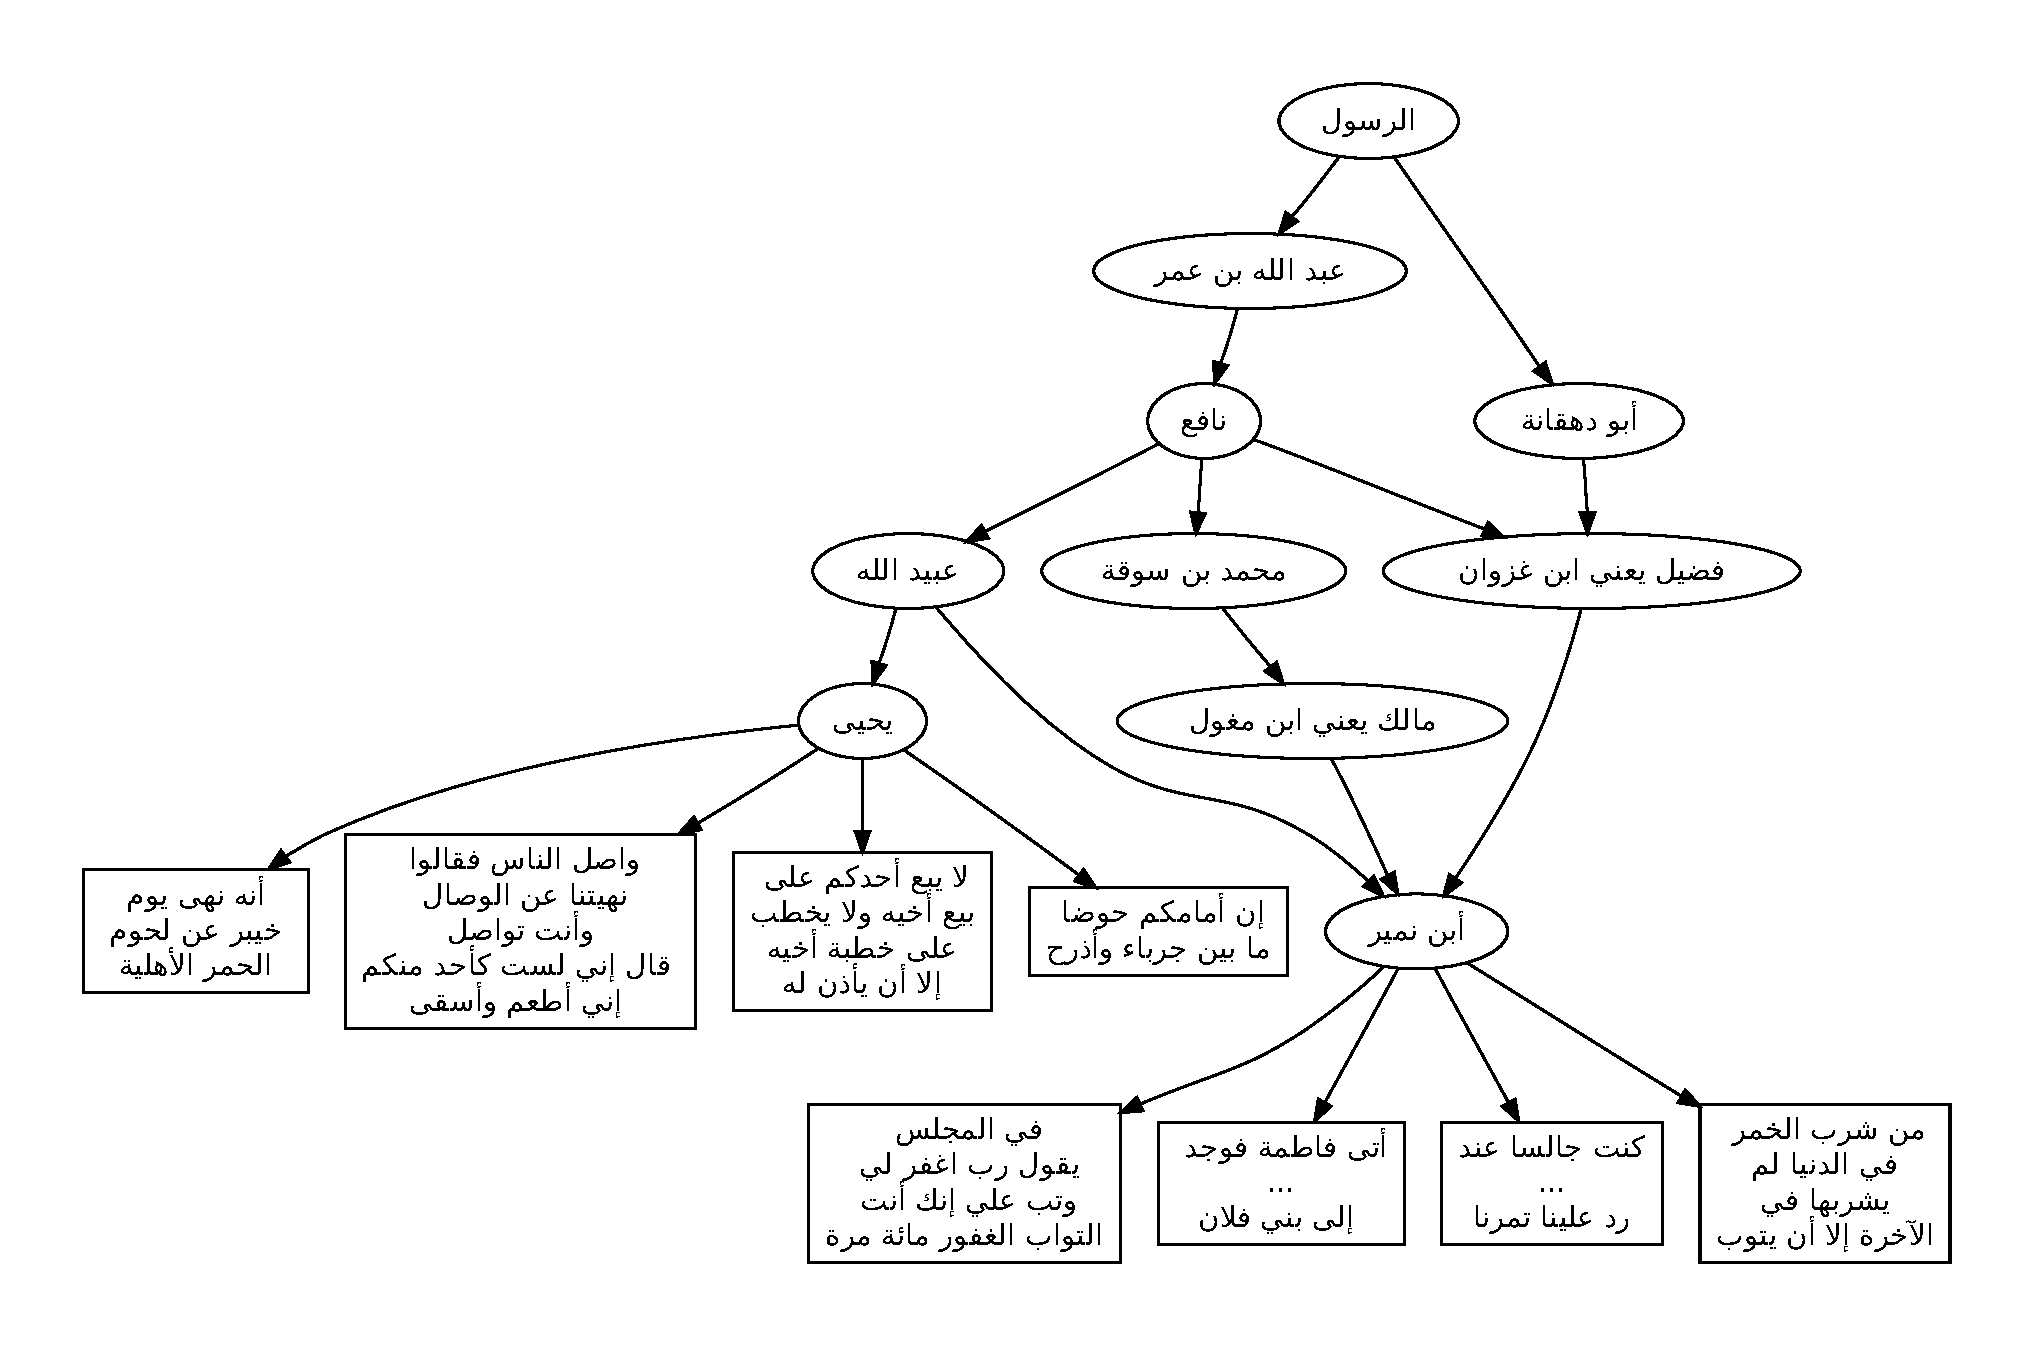
\includegraphics{figs/narrator_chain_output.pdf}}
\caption{Directed acyclic graph representing a partial order 
    relation between narrators extracted using ATSarf}
\label{f:narrators} 
}
\end{figure}

The directed acyclic graph (DAG) 
in Figure~\ref{f:narrators} shows a partial order relation (POR) between
narrators.
We automatically extracted the POR from hadith text 
documents.
The nodes in boxes are the \RL{matn} of the hadith, 
and the other nodes are the narrators.
Given a set of chains of narrators similar to 
Figure~\ref{f:exhadith} we formed the DAG using graph algorithms 
that merged equal names in the chains. 
This partial order graph is instrumental to automate
localizing narrators in biography documents and
segmenting biography documents.

Given that a biography will discuss a narrator and mention
his professors and students,
we can segment the biographies with a graph coloring algorithm 
that traverses the text and colors the POR whenever
a name is found. 
We modify the color when we move in the graph 
far away from the last name we colored.

Once the biographies are analyzed, one can annotate
the POR with qualifiers of the narrators that reflect
their authenticity. 
One can also annotate the POR with the locations and 
the time they lived in. 
Then One can compute a time and location overlap
check to discover inconsistent narrations.
We can also perform several interesting checks using 
this POR on its own such as checking for the effect of
one narrator on the hadith literature. 

These preliminary results serve as a good proof of concept to our 
hypothesis. They also confirm that our approach performs better than 
currently existing techniques from Sakhr~\cite{Sak09},
Basis~\cite{Bas09} and open source 
tools~\cite{Col09,Otakar:07,Tim04}.

We find evidence in our current results that features 
of the Arabic language such as the hierarchical structure of
names can be used to simplify the morphological analysis
needed to extract the partial order graph. 
Publications about these results are pending acceptance in 
related NLP conferences. 


\section{Goals for next year}
\label{s:nextyear}

Our first year of research on 
Arabic text mining proved to be 
fruitful. 
For the next year, we expect to complete the hadith literature case 
study and to start and complete the security case study. 
We will package the components built during the development of these 
case studies as independent text mining entity and relational 
extractors to be included in the framework.
Moreover, we expect to be able to enhance the morphological analyzer in 
terms of speed, accuracy, and semantic capabilities. 
We will also investigate methods to extend the internal structures 
of our analyzer to be able to represent a formal linguistic
computational model of the Arabic language. 
In what follows we describe our expectations in terms of each case-study.

\subsection{Literature authentication case study}
\label{s:design:lit}

%\begin{figure}[tb]
\begin{figure}
\center{
\resizebox{.75\columnwidth}{!}
{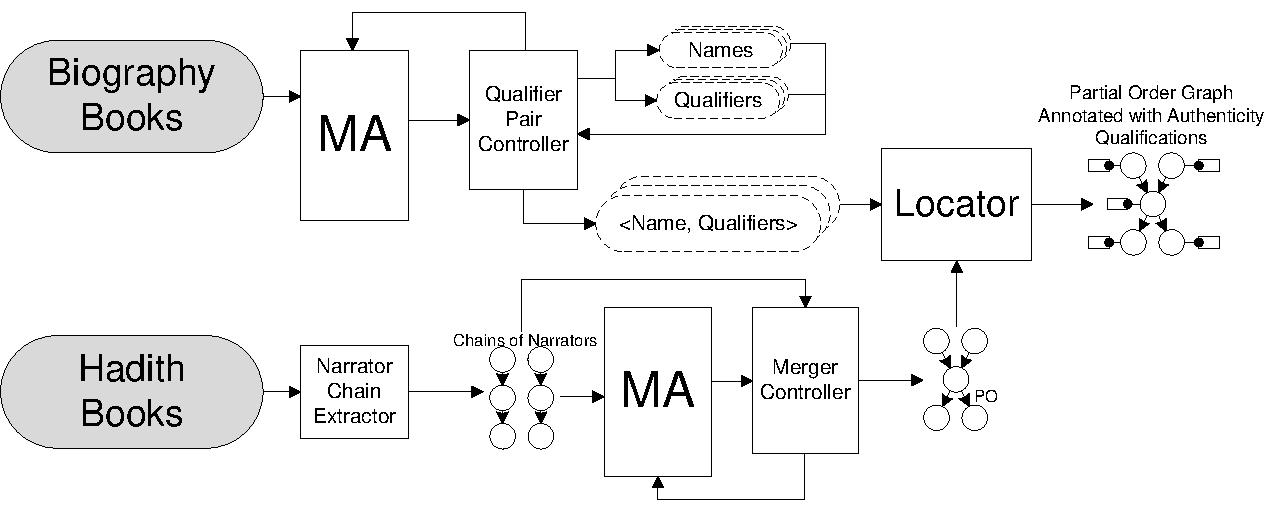
\includegraphics{figs/literature_case-study1.pdf}
} 
\caption{Diagram for the literature case study }
\label{f:literature}
}
\end{figure}

The diagram in Figure~\ref{f:literature} describes our 
high level vision for what the literature case study
will look like in the framework to be developed. 
The boxes represent 
computational blocks provided by the framework, 
ovals represent data blocks which are mainly the 
inputs and the outputs of the computational blocks. 
Dotted data blocks represent intermediate results,
and solid and shaded blocks represent the initial input 
and the final output respectively. 

The computational components can be direct components of the framework
or custom user components built from other components.
We feed the hadith books to a user Narrator Chain Extractor
component that we have built using finite state machines (described in the attached paper).
We  obtain a set of chains
of narrators that we feed to a morphological analyzer (MA) 
component controlled by a merger controller. 
The merger controller will look at the morphological analysis
of the narrator names and will decide to merge two narrators in 
one graph node in case they were morphologically equal. 
It will also give feedback to the MA component to stop the
analysis when a it reaches a satisfactory result.
We consider this graph as a partial order relation between 
narrators where a narrator precedes another narrator if 
he narrated from him. 

The biography books are fed to another MA unit controlled by 
a name and qualification pair controller that generates a 
map consisting of pairs of narrator names associated with 
qualifications. 
Then the graph of narrators and the narrator qualification map
are both processed through a locator component that computes
a graph coloring routine to color the graph of narrators. 
The color changes when two consecutive narrators are far away
from each other in the text. 
The locator then looks at connected subgraphs of the same color,
and finds a median node in each of them to be the narrator 
associated with the qualifiers of the color. 
Then the locator also annotates the narrator with the 
corresponding qualifications. 
The result is an annotated partial order graph of narrators
with authentication qualification annotations. 

\subsection{Security case study}
\label{s:design:sec}

%\begin{figure}[tb]
\begin{figure}
\center{
\resizebox{.8\columnwidth}{!}
{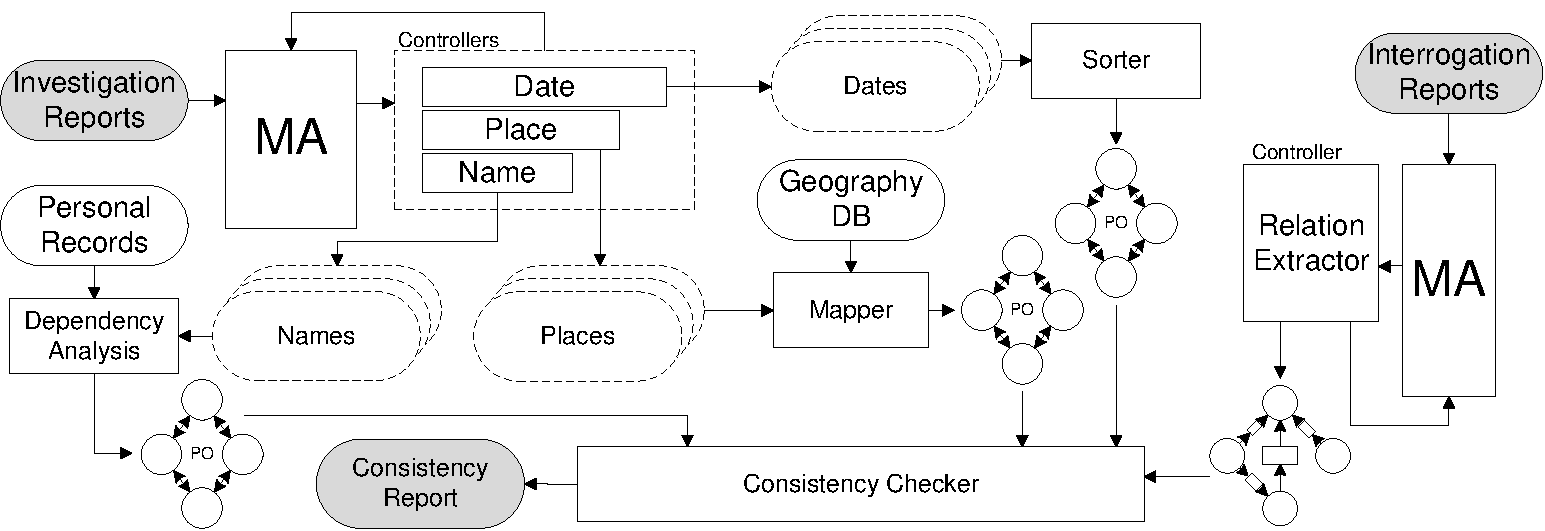
\includegraphics{figs/security_case-study.pdf}
}
\caption{Diagram for the security case study}
\label{f:security}
}
\end{figure}


The diagram in Figure~\ref{f:security} describes our 
high level vision for what the solution of the 
security case study
will look like in the framework. 
The inputs are two separate sets of documents. 
The first set includes crime scene investigation reports, 
and the second set includes a 
interrogation reports with crime suspects as well as 
a database of previous interrogation reports. 
We will first try our system on dummy data with seeded relations.
Once the system is ready, we will deliver it to local police
and intelligence agencies to try it out on real digitized 
reports. 

The system also takes as input a database of geographical
locations and a database of personal records. 
The aim is to check for inconsistencies in the interrogation
reports and to identify possible connections between the suspects
and the crime scene. 

An MA with date, place, and name extraction controller extracts
names, dates and places from the investigation reports. 
We pass the dates to a sorting component to produce $G_D$ 
a partial order graph between the dates. 
We look up the names in the personal records database and find out
$G_N$ a family dependency graph between the names. 
We pass the places to a mapper that builds another $G_G$,
a graph relating the places using a geographical database. 

We pass the interrogation reports to an MA with a relation 
extraction controller that builds $G_R$. 
The graph $G_R$ relates the interrogated suspects
to each other, to places, and to dates based on a simple
neighborhood threshold computed using a statistical feature. 

We feed $G_D, G_F, G_G,$ and $G_R$   
to a consistency checker.
The consistency checker considers the three dimensions 
$N$ names, $G$ locations, and $D$ dates and projects $G_R$
over each one of them.
For each dimension $k$, it computes a local measure 
$\alpha_k$ of how much $G_R|_k$ simulates $G_k$. 
It flags the components in the graph where the accumulated 
measure $\alpha= \Sigma_{k\in\{D,N,G\}} \alpha_k$ is
below a threshold $\theta$ as inconsistent. 

\section{Budget for year 2011}
\label{s:budget}

In the table below we summarize our itemized budget for year 2011. 

\begin{table}[ht]
\begin{tabular}{l r}

 \hline
 One part-time research assistant for 8 month: LL. 750K/month  & LL. 6000K  \\
 Arabic Corpus License & LL. 1500K \\
Miscellaneous  & LL. 500K \\
\hline
 Total  & LL. 8000K \\
 \hline
\end{tabular} 
\end{table}


\section{Submission to: ``ACL/HTL 2011"}
\label{s:paper}

We have submitted the attached paper to the “The 49h Annual Meeting of the Association for Computational Linguistics: Human Language Technologies (ACL/HLT 2011)”. The paper is entitled: “Case-based Arabic Morphological Analysis”.

%\bibliography{adnan_refs}
%\bibliographystyle{ieeetr}
\bibliographystyle{abbrvnat}
%\bibliographystyle{ieeetr}
{\small
\bibliography{fzAr}  
}


\end{document}
